\documentclass[main.tex]{subfiles}

\begin{document}
	
	
	\subsection{Error dynamics}
	
	The system equations for the neutral bit walk model are given by:
	
	\begin{equation}
	\begin{aligned}
	\chi \Pi \Theta ' =  &- \mathcal{M}_b(\Theta-\langle\Theta \rangle_1)-\frac{{{\mathcal{M}_b}{F_1} + {\mathcal{M}_1}\left( {\eta \Pi  - {\mathcal{F}_b}} \right)}}{{\eta \Pi }}\left( {{\langle{\rm{\Theta }} \rangle_1} - {\langle{\rm{\Theta }} \rangle_{2}}} \right)
	\\
	&+\frac{\chi }{\eta }{\mathcal{F}_b}\left( {{\rm{\Theta }} - {{\rm{\Theta }}_1}} \right)
	- \frac{\chi }{\eta }{\mathcal{F}_1}\left( {{{{{\rm{\Theta }}} - {{\rm{\Theta }}_1}}} - \frac{{{{\rm{\Theta }}_1} - {{\rm{\Theta }}_{2}}}}{{{\varkappa _{2}}}}} \right)
	\\
	&- \frac{{{\mathcal{M}_b}{\mathcal{F}_r} + (\eta \Pi  - {F_b}){\mathcal{M}_r}}}{{\eta \Pi }}{\Gamma _{\Theta}} - \frac{\chi }{\eta }{\mathcal{F}_r}\Gamma_{\!\Theta}' + W,
	\\
	\chi \Pi \Phi ' =  &- {\mathcal{M}_b}\left( {\Phi  - {\langle{\rm{\Phi }} \rangle_1}} \right)-\frac{{{\mathcal{M}_b}{F_1} + {\mathcal{M}_1}\left( {\eta \Pi  - {F_b}} \right)}}{{\eta \Pi }}\left( {{\langle{\rm{\Phi }} \rangle_1} - {\langle{\rm{\Phi }} \rangle_{2}}} \right)
	\\
	&+\frac{\chi }{\eta }{\mathcal{F}_b}\left( {{\rm{\Phi }} - {{\rm{\Phi }}_1}} \right)
	- \frac{\chi }{\eta }{\mathcal{F}_1}\left( {{{{{\rm{\Phi }}} - {{\rm{\Phi }}_1}}} - \frac{{{{\rm{\Phi }}_1} - {{\rm{\Phi }}_{2}}}}{{{\varkappa _{2}}}}} \right)
	\\
	&+ \left( {\frac{\chi }{\eta }\frac{{{\mathcal{F}_r}\Theta '\cos \Theta }}{{{{\left( {\sin \Theta } \right)}^2}}} - \frac{{{\mathcal{M}_b}{\mathcal{F}_r} + {\mathcal{M}_r}\left( {\eta \Pi  - {\mathcal{F}_b}} \right)}}{{\eta \Pi \sin \Theta }}} \right){\Gamma _{\Phi}} - \frac{\chi }{\eta }\frac{{{\mathcal{F}_r}}}{{\sin \Theta }}\Gamma_{\!\Phi}',
	\end{aligned}
	\label{eq:neutralbitwalkmodelfordesign}
	\end{equation}
	
	
	where the term related to the weight of the BHA is included in the first equation and is given by $W = -\frac{\mathcal{M}_b \mathcal{F}_w + (\eta \Pi - \mathcal{F}_b)\mathcal{M}_w}{\eta \Pi}\Upsilon \sin \langle\Theta\rangle_1 -\frac{\chi}{\eta}\mathcal{F}_w (\Theta - \Theta_1)\Upsilon \cos \langle\Theta\rangle_1$ and $\Upsilon$ is the normalized weight of the BHA.
	
	From Equation \eqref{eq:neutralbitwalkmodelfordesign}, the states of the system can be defined as:
	
	\begin{equation}
	x_\Theta = \begin{bmatrix}
	\Theta \\
	\langle \Theta \rangle_1\\
	\langle\Theta \rangle_2 
	\end{bmatrix}, \qquad
	x_\Phi = \begin{bmatrix}
	\Phi \\
	\langle \Phi \rangle_1\\
	\langle\Phi \rangle_2 
	\end{bmatrix}.
	\end{equation}
	
	The system's output equations are given corresponding to measurements not exactly at the bit, but as the orientation of the BHA at locations between the stabilizers and given by:
	
	\begin{align}
		y_\Theta &= C_\Theta x_\Theta + D_\Theta \Gamma_\Theta + E \Upsilon \sin \langle \Theta \rangle_1 \label{eq:output1}\\
		y_\Phi &= C_\Phi x_\Phi + D_\Phi \frac{\Gamma_\Phi}{\sin \Theta}.\label{eq:output2}		
	\end{align}
	
	If it is assumed that both the inclination and the azimuth sensors are at the same location then $C_\Theta = C_\Phi$ and $D_\Theta = D_\Phi$.

	The input transformation on Equation \eqref{eq:decouplinginputtransformation2} is proposed in order to achieve decoupling of the system, it has to be noticed that the transformation on $\Gamma_\Phi$ depends on the estimate $\check{\Theta}$ of the inclination, if there is no access to measurements of the orientation of the borehole at the bit.
	
	\begin{equation}
	\begin{bmatrix}
	\Gamma_{\!\Theta}^* \\ \Gamma_{\!\Phi}^* 	
	\end{bmatrix} :=  \begin{bmatrix} 1 & 0 \\ 0 & \frac{1}{\sin \check{\Theta}}\end{bmatrix} \begin{bmatrix}\Gamma_{\!\Theta} \\ \Gamma_{\!\Phi} \end{bmatrix}, \qquad \text{for } \Theta\in (0,\; \pi),
	\label{eq:decouplinginputtransformation2}
	\end{equation}
	
	Since the input transformation does not change the structure of the first equation in \eqref{eq:neutralbitwalkmodelfordesign}, only the second equation is shown and is given by:
	
	\begin{equation}
	\begin{aligned}
	\chi \Pi \Phi ' =  &- {\mathcal{M}_b}\left( {\Phi  - {\langle{\rm{\Phi }} \rangle_1}} \right)-\frac{{{\mathcal{M}_b}{F_1} + {\mathcal{M}_1}\left( {\eta \Pi  - {F_b}} \right)}}{{\eta \Pi }}\left( {{\langle{\rm{\Phi }} \rangle_1} - {\langle{\rm{\Phi }} \rangle_{2}}} \right)
	\\
	&+\frac{\chi }{\eta }{\mathcal{F}_b}\left( {{\rm{\Phi }} - {{\rm{\Phi }}_1}} \right)
	- \frac{\chi }{\eta }{\mathcal{F}_1}\left( {{{{{\rm{\Phi }}} - {{\rm{\Phi }}_1}}} - \frac{{{{\rm{\Phi }}_1} - {{\rm{\Phi }}_{2}}}}{{{\varkappa _{2}}}}} \right)
	\\
	&+ \left( {\frac{\chi }{\eta }\frac{{{\mathcal{F}_r}\Theta '\cos \Theta \sin \check{\Theta} }}{{{{\left( {\sin \Theta } \right)}^2}}}
		- \frac{{{(\mathcal{M}_b}{\mathcal{F}_r} + {\mathcal{M}_r}\left( {\eta \Pi  - {\mathcal{F}_b}}) \right)\sin\check{\Theta}}}{{\eta \Pi \sin \Theta }} - \frac{\chi }{\eta }\frac{{{\mathcal{F}_r}\check{\Theta} '\cos \check{\Theta}}}{{{{\left( {\sin \Theta } \right)}}}}} \right){\Gamma _{\Phi}^*}
	- \frac{\chi }{\eta }\frac{{{\mathcal{F}_r \sin \check{\Theta}}}}{{\sin \Theta }}\Gamma_{\!\Phi}^{* '}.
	\end{aligned}
	\label{neutralbitwalkphi}
	\end{equation}
	

	and the system equations can be rewritten as:

	\begin{align}
		\begin{bmatrix}
			x_\Theta' \\
			x_\Phi'
		\end{bmatrix} =&
		\begin{bmatrix}
			A_0 & 0 \\
			0 & A_0
		\end{bmatrix}
		\begin{bmatrix}
			x_\Theta(\xi) \\
			x_\Phi(\xi)
		\end{bmatrix} + 
		\begin{bmatrix}
		A_1 & 0 \\
		0 & A_1
		\end{bmatrix}
		\begin{bmatrix}
		x_\Theta(\xi_1) \\
		x_\Phi(\xi_1)
		\end{bmatrix} +
		\begin{bmatrix}
		A_2 & 0 \\
		0 & A_2
		\end{bmatrix}
		\begin{bmatrix}
		x_\Theta(\xi_2) \\
		x_\Phi(\xi_2)
		\end{bmatrix} \nonumber\\
		+&
	   \begin{bmatrix}
		B_{0\Theta} & 0\\
		0 & B_{0\Phi}
		\end{bmatrix} 
		\begin{bmatrix}
		\Gamma_\Theta^* \\
		\Gamma_\Phi^*
		\end{bmatrix} +
		\begin{bmatrix}
		B_{1\Theta} & 0\\
		0 & B_{1\Phi}
		\end{bmatrix} 
		\begin{bmatrix}
		\Gamma_\Theta^{*'} \\
		\Gamma_\Phi^{*'}
		\end{bmatrix} + 
		\begin{bmatrix}
		BW \\
		0
		\end{bmatrix},
		\label{eq:systemstatespace}	
	\end{align}
	
	where the matrices and vectors $A_0$, $A_1$, $A_2$, $B$, $B_{0i}$ and $B_{1i}$, for $i = \Theta, \Phi$, are given by:
	
	\begin{align}
		A_{0}&= \frac{1}{\chi\Pi}\begin{bmatrix}
		-\mathcal{M}_b+ \frac{\chi}{\eta}(\mathcal{F}_b-\mathcal{F}_1)     & \mathcal{M}_b-\mathcal{M}_1+\frac{\mathcal{F}_b\mathcal{M}_1-\mathcal{F}_1\mathcal{M}_b}{\eta\Pi}            & \mathcal{M}_1+\frac{(-\mathcal{F}_b\mathcal{M}_1+\mathcal{F}_1\mathcal{M}_b)}{\eta\Pi} \\ 
		\chi\Pi    & 0             & 0            \\
		0     & 0             & 0            \\
		\end{bmatrix}, \nonumber \\\nonumber
		\\ \nonumber
		A_{1}&= \frac{1}{\chi\Pi}\begin{bmatrix}
		\frac{\chi}{\eta}(\mathcal{F}_1+\frac{\mathcal{F}_1}{\varkappa_2}-{\mathcal{F}_b})     & 0             & 0            \\
		-\chi\Pi     & 0             & 0            \\
		\frac{\chi\Pi}{\varkappa_2}    & 0             & 0            \\
		\end{bmatrix}, \qquad
		A_{2}= \frac{1}{\chi\Pi}\begin{bmatrix}
		-\frac{\chi \mathcal{F}_1}{\eta\varkappa_2}     & 0             & 0            \\
		0     & 0             & 0            \\
		-\frac{\chi\Pi}{\varkappa_2}     & 0             & 0            \\
		\end{bmatrix},\nonumber
		\\\nonumber
		\\ \nonumber
		B_{0\Theta}&= \frac{1}{\chi\Pi}\begin{bmatrix}
			- \frac{{{\mathcal{M}_b}{\mathcal{F}_r} + (\eta \Pi  - {F_b}){\mathcal{M}_r}}}{{\eta \Pi }},   & 0,             & 0           \\
		\end{bmatrix}^{T} , \qquad
		B_{1\Theta}= \frac{1}{\chi\Pi}\begin{bmatrix}
		-\frac{\chi}{\eta}\mathcal{F}_r ,    & 0,            & 0            \\
		\end{bmatrix}^{T}, 
		\\\nonumber
		\\ \nonumber
		B_{0\Phi}&= \frac{1}{\chi\Pi}\begin{bmatrix}
		{\frac{\chi }{\eta }\frac{{{\mathcal{F}_r}\Theta '\cos \Theta \sin \check{\Theta} }}{{{{\left( {\sin \Theta } \right)}^2}}}
			- \frac{{{(\mathcal{M}_b}{\mathcal{F}_r} + {\mathcal{M}_r}\left( {\eta \Pi  - {\mathcal{F}_b}}) \right)\sin\check{\Theta}}}{{\eta \Pi \sin \Theta }} - \frac{\chi }{\eta }\frac{{{\mathcal{F}_r}\check{\Theta} '\cos \check{\Theta}}}{{{{\left( {\sin \Theta } \right)}}}}},   & 0,             & 0           \\
		\end{bmatrix}^{T} \nonumber \\ \nonumber
		\\ \nonumber
		B_{1\Phi}&= \frac{1}{\chi\Pi}\begin{bmatrix}
		-\frac{\chi}{\eta}\mathcal{F}_r\frac{\sin \check{\Theta}}{\sin \Theta} ,    & 0,            & 0            \\
		\end{bmatrix}^{T}, \qquad B = \begin{bmatrix}1 & 0 & 0\end{bmatrix}^T.
	\end{align}
	
	After the input transformation, the output equations are given by:
	
	\begin{align}
		y_\Theta &= C_\Theta x_\Theta + D_\Theta \Gamma_\Theta^* + E W_y, \label{eq:output12}\\
		y_\Phi &= C_\Phi x_\Phi + D_\Phi \Gamma_\Phi^*	\frac{\sin \check{\Theta}}{\sin \Theta}	.\label{eq:output22},	
	\end{align}
	
	where the gravity related term in $y_\Theta$ has been renamed to $E W_y$, with $W_y = \Upsilon \sin \langle \Theta \rangle_1$ to simplify notation, and take them also as a quasi-constant perturbation. It can be seen that the system equations are complex, especially because of the fact that the terms related to the derivatives of the inclination and its estimate are affecting the azimuth dynamics. This is mainly due to the difference between $\Theta$ and $\check{\Theta}$. For the zero bit walk case (as considered here), this complexity vanishes when $\check{\Theta} = \Theta$. Assuming that we will be able to design an observer that indeed provides (asymptotically) such correct estimate of the inclination, the structure of the controller will be designed for the case when this condition is met.
	
	\begin{figure}[h]\centering
		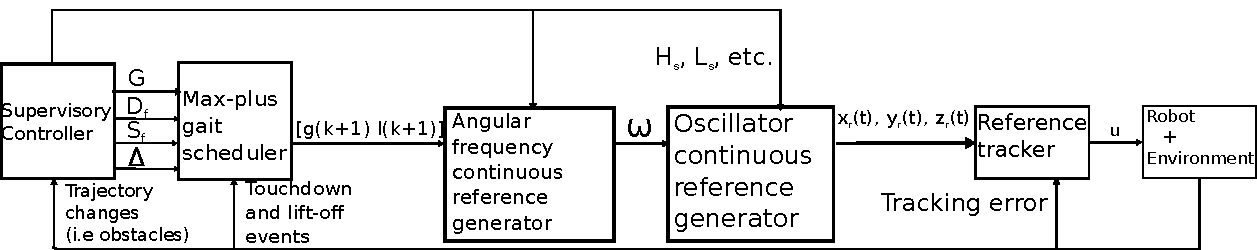
\includegraphics[width=0.65\textwidth]{ControlStrategy.pdf}
		\caption{Control strategy.
			\label{fig:ControlStrat} }
	\end{figure}
	
		
	The total control scheme proposed here is depicted schematically in Figure \ref{fig:ControlStrat}. In order to combine the (transformed) RSS force inputs $\Gamma_i^*$ for $i = \Theta, \Phi$ and their derivatives, the following transformation is proposed:
	
	\begin{equation}
		B u_i = B_{0i}\Gamma_i^* + B_{1i}\Gamma_i^{*'}, 	\label{eq:inputs1}\\
	\end{equation}
	
	where $B = \begin{bmatrix} 1 & 0 & 0\end{bmatrix}^T$ and vectors $B_{0i}$ and $B_{1i}$ correspond to the 3 by 1 vectors related to the inputs of the azimuth and the inclination.
	
	This would fully replace the terms related to $\Gamma_i^*$ and their derivative in the dynamics given by \eqref{eq:systemstatespace} with $Bu$. However, it is not possible to use the input filter as in \eqref{eq:inputs1} here, since vectors $B_{0\Phi}$ and $B_{1\Phi}$ depend on $\Theta$, which is not known to the controller, since it can not be measured. To overcome this, the design of this input filter will be done for the case when $\check{\Theta} = \Theta$, i.e.
	
	\begin{align}
	\Gamma_{i}^{*'} = -\frac{\mathcal{M}_b \mathcal{F}_r + (\eta \Pi - \mathcal{F}_b)\mathcal{M}_r}{\chi \Pi \mathcal{F}_r}\Gamma_{i}^{*} - \frac{\eta \Pi}{\mathcal{F}_r}u_i. \label{eq:filter1} 	
	\end{align}	
	
	Herein, $u_i$ is a new control input, comprised of the sum of the feedforward and feedback inputs given by $u_i = v_i + u_{ri}$. The stability of the filter is guaranteed as long as $\frac{B_{0i}}{B_{1i}} > 0$. It can be seen, that considering only uncertainty for the weight on bit, this condition is met up to a certain value of $\Pi$. It was proven in \cite{Kremers2013} that this value corresponds to the situation where the system is minimum-phase, this is as long as $\Pi < \Pi_{nmp}$, which is the focus of this work. In \eqref{eq:filter1}, the feedforward input $u_{ri}$ is defined based on the inverse dynamics of the system for a reference trajectory:
	
	\begin{equation}
	u_{ri} = B^T (x'_{ri}(\xi) - A_0 x_{ri}(\xi) - A_1 x_{ri}(\xi_1) - A_2 x_{ri}(\xi_2)).
	\label{eq:feedforward}
	\end{equation}
	
	It is important to mention that the gravity related term in the inclination dynamics (W in \eqref{eq:neutralbitwalkmodelfordesign}), is omitted from the feedforward design since it can be considered as a quasi-constant(unknown) disturbance, which can be dealt with by implementing integral action in the control structure. Furthermore, this feedforward is designed again for the case when $\check{\Theta} = \Theta$. Due to this simplification of the feedforward design, a (transient) error is introduced to the system, which will be taken into account explicitly in the resulting error dynamics later.

	
	If the input filters are substituted in Equation \eqref{eq:systemstatespace}, then the system dynamics are given by:
	
	\begin{align}
	\begin{bmatrix}
	x_\Theta' \\
	x_\Phi'
	\end{bmatrix} =&
	\begin{bmatrix}
	A_0 & 0 \\
	0 & A_0
	\end{bmatrix}
	\begin{bmatrix}
	x_\Theta(\xi) \\
	x_\Phi(\xi)
	\end{bmatrix} + 
	\begin{bmatrix}
	A_1 & 0 \\
	0 & A_1
	\end{bmatrix}
	\begin{bmatrix}
	x_\Theta(\xi_1) \\
	x_\Phi(\xi_1)
	\end{bmatrix} +
	\begin{bmatrix}
	A_2 & 0 \\
	0 & A_2
	\end{bmatrix}
	\begin{bmatrix}
	x_\Theta(\xi_2) \\
	x_\Phi(\xi_2)
	\end{bmatrix} \nonumber\\
	+& \begin{bmatrix}
	0 & 0 \\
	0 & B\frac{\mathcal{F}_r}{\eta \Pi \sin \Theta} \bigg( \frac{\Theta' \cos \Theta \sin \check{\Theta}}{\sin \Theta}  - \check{\Theta}' \cos \check{\Theta}\bigg)
	\end{bmatrix}
	\begin{bmatrix}
	\Gamma_\Theta^* \\
	\Gamma_\Phi^*
	\end{bmatrix} + \begin{bmatrix}
	B & 0 \\
	0 & B\frac{\sin \check{\Theta}}{\sin \Theta}
	\end{bmatrix}
	\begin{bmatrix}
	u_\Theta \\
	u_\Phi
	\end{bmatrix} +
	\begin{bmatrix}
	BW \\
	0
	\end{bmatrix}.
	\label{eq:systemstatespace2}	
	\end{align}
	
	
	In the case of the inclination dynamics, the input filter successfully makes the terms related to $\Gamma_\Theta^*$ disappear from the equation. On the other hand, in the equation related to the azimuth dynamics, one term related to $\Gamma_\Phi^*$ remains due to the mismatch between $\check{\Theta}$ and $\Theta$. Moreover, in \eqref{eq:systemstatespace2} there is a nonlinear factor multiplied by input $u_\Phi$. If the input filters in \eqref{eq:filter1} are included in the equation, the system dynamics can be rewritten as follows:
	
	\begin{align}
	\begin{bmatrix}
	x_\Theta' \\
	\Gamma_\Theta^{*'} \\
	x_\Phi' \\
	\Gamma_\Phi^{*'} 
	\end{bmatrix} =&
	\begin{bmatrix}
	A_0 & 0 & 0 & 0\\
	0 & -b_0 & 0 & 0 \\
	0 & 0 & A_0 & B\alpha(\Theta,\check{\Theta},\Theta',\check{\Theta}') \\
	0 & 0 & 0 & -b_0
	\end{bmatrix}
	\begin{bmatrix}
	x_\Theta(\xi) \\
	\Gamma_\Theta^{*}(\xi) \\
	x_\Phi(\xi) \\
	\Gamma_\Phi^{*} (\xi)
	\end{bmatrix} + 
	\begin{bmatrix}
	A_1 & 0 & 0 & 0\\
	0 & 0 & 0 & 0 \\
	0 & 0 & A_1 & 0 \\
	0 & 0 & 0 & 0 \\
	\end{bmatrix}
	\begin{bmatrix}
	x_\Theta(\xi_1) \\
	\Gamma_\Theta^{*}(\xi_1) \\
	x_\Phi(\xi_1) \\
	\Gamma_\Phi^{*} (\xi_1)
	\end{bmatrix} +
	\begin{bmatrix}
	A_2 & 0 & 0 & 0 \\
	0 & 0 & 0 & 0 \\
	0 & 0 & A_2 & 0 \\
	0 & 0 & 0 & 0 \\
	\end{bmatrix}
	\begin{bmatrix}
	x_\Theta(\xi_2) \\
	\Gamma_\Theta^{*}(\xi_2) \\
	x_\Phi(\xi_2) \\
	\Gamma_\Phi^{*} (\xi_2)
	\end{bmatrix}\nonumber \\ 
	&+
	\begin{bmatrix}
	B & 0 \\
	-b_1 & 0 \\
	0 & B \frac{\sin \check{\Theta}}{\sin \Theta} \\
	0 & -b_1
	\end{bmatrix}
	\begin{bmatrix}
	u_\Theta \\
	u_\Phi
	\end{bmatrix} +
	\begin{bmatrix}
	BW \\
	0 \\
	0 \\
	0
	\end{bmatrix}.
	\end{align}
	
	where:
	
	\begin{equation}
		b_0 = \frac{\mathcal{M}_b \mathcal{F}_r + (\eta \Pi - \mathcal{F}_b)\mathcal{M}_r}{\chi \Pi \mathcal{F}_r}, \quad b_1 = \frac{\eta \Pi}{\mathcal{F}_r}, \quad \alpha (\Theta,\check{\Theta},\Theta',\check{\Theta}') = \frac{\mathcal{F}_r}{\eta \Pi \sin \Theta} \bigg( \frac{\Theta' \cos \Theta \sin \check{\Theta}}{\sin \Theta}  - \check{\Theta}' \cos \check{\Theta}\bigg). \label{eq:Constants}
	\end{equation}
	
	It has to be noticed that $\alpha$ depends on the states $\Theta$ and $\check{\Theta}$, and their derivatives. To simplify notation, $\alpha$ will be written  instead of $\alpha(\Theta,\check{\Theta}, \Theta', \check{\Theta}')$. From these equations, the error dynamics of the system (with the error defined as $e_i = x_i - x_{ri}$) are obtained in \eqref{eq:errordynamics}, using for the feedforward the expression given in \eqref{eq:feedforward} and the control input decomposition $u_i = u_{ri} + v_i$:
		
	\begin{align}
		\begin{bmatrix}
		e_\Theta' \\
		\Gamma_\Theta^{*'} \\
		e_\Phi' \\
		\Gamma_\Phi^{*'}
		\end{bmatrix} =&
		\begin{bmatrix}
		A_0 & 0 & 0 & 0\\
		0 & -b_0 & 0 & 0 \\
		0 & 0 & A_0 & B \alpha \\
		0 & 0 & 0 & -b_0
		\end{bmatrix}
		\begin{bmatrix}
		e_\Theta(\xi) \\
		\Gamma_\Theta^{*} (\xi) \\
		e_\Phi(\xi) \\
		\Gamma_\Phi^{*} (\xi) 
		\end{bmatrix} + 
		\begin{bmatrix}
		A_1 & 0 & 0 & 0\\
		0 & 0 & 0 & 0 \\
		0 & 0 & A_1 & 0 \\
		0 & 0 & 0 & 0 
		\end{bmatrix}
		\begin{bmatrix}
		e_\Theta(\xi_1) \\
		\Gamma_\Theta^{*} (\xi_1) \\
		e_\Phi(\xi_1) \\
		\Gamma_\Phi^{*} (\xi_1) 
		\end{bmatrix} +
		\begin{bmatrix}
		A_2 & 0 & 0 & 0\\
		0 & 0 & 0 & 0 \\
		0 & 0 & A_2 & 0 \\
		0 & 0 & 0 & 0 
		\end{bmatrix}
		\begin{bmatrix}
		e_\Theta(\xi_2) \\
		\Gamma_\Theta^{*} (\xi_2) \\
		e_\Phi(\xi_2) \\
		\Gamma_\Phi^{*} (\xi_2) 
		\end{bmatrix} \nonumber\\
		 &+ \begin{bmatrix}
		 B & 0 \\
		 -b_1 & 0 \\
		 0 & B\bigg( \frac{\sin \check{\Theta}}{\sin \Theta}\bigg) \\
		 0 & -b_1 
		 \end{bmatrix}
		\begin{bmatrix}
		v_\Theta \\
		v_\Phi
		\end{bmatrix} + 
		\begin{bmatrix}
		0 \\
		-b_1 u_{r\Theta} \\
		B\bigg( \frac{\sin \check{\Theta}}{\sin \Theta} - 1 \bigg) u_{r\Phi} \\
		-b_1 u_{r\Phi}
		\end{bmatrix}+
		\begin{bmatrix}
		BW \\
		0 \\
		0 \\
		0
		\end{bmatrix}.
		\label{eq:errordynamics}
	\end{align}
	
	In a similar way, if an input filter as in equation \eqref{eq:filter1} is designed based on the feedforward input, the following equation can be obtained:
	
	\begin{equation}
			\Gamma_{id}^{*'} = -\frac{\mathcal{M}_b \mathcal{F}_r + (\eta \Pi - \mathcal{F}_b)}{\chi \Pi \mathcal{F}_r}\Gamma_{id}^{*} - \frac{\eta \Pi}{\mathcal{F}_r}u_{ri}, \label{eq:filter2} 	
	\end{equation}
	
	where $\Gamma_{id}^*$ is a desired input of the RSS corresponding to the feedforward input. Then, an error coordinate for the transformed input $\Gamma_i^*$ can be defined as $\Delta \Gamma^*_{i} = \Gamma_i^* - \Gamma_{id}^*$. Then equation \eqref{eq:errordynamics} can be rewritten as:
	
	 \begin{align}
	 \begin{bmatrix}
	 e_\Theta' \\
	 \Delta \Gamma_\Theta^{*'} \\
	 e_\Phi' \\
	 \Delta \Gamma_\Phi^{*'}
	 \end{bmatrix} =&
	 \begin{bmatrix}
	 A_0 & 0 & 0 & 0\\
	 0 & -b_0 & 0 & 0 \\
	 0 & 0 & A_0 & B \alpha \\
	 0 & 0 & 0 & -b_0
	 \end{bmatrix}
	 \begin{bmatrix}
	 e_\Theta(\xi) \\
	 \Delta \Gamma_\Theta^{*} (\xi) \\
	 e_\Phi(\xi) \\
	 \Delta \Gamma_\Phi^{*} (\xi) 
	 \end{bmatrix} + 
	 \begin{bmatrix}
	 A_1 & 0 & 0 & 0\\
	 0 & 0 & 0 & 0 \\
	 0 & 0 & A_1 & 0 \\
	 0 & 0 & 0 & 0 
	 \end{bmatrix}
	 \begin{bmatrix}
	 e_\Theta(\xi_1) \\
	 \Delta \Gamma_\Theta^{*} (\xi_1) \\
	 e_\Phi(\xi_1) \\
	 \Delta \Gamma_\Phi^{*} (\xi_1) 
	 \end{bmatrix} +
	 \begin{bmatrix}
	 A_2 & 0 & 0 & 0\\
	 0 & 0 & 0 & 0 \\
	 0 & 0 & A_2 & 0 \\
	 0 & 0 & 0 & 0 
	 \end{bmatrix}
	 \begin{bmatrix}
	 e_\Theta(\xi_2) \\
	 \Delta \Gamma_\Theta^{*} (\xi_2) \\
	 e_\Phi(\xi_2) \\
	 \Delta \Gamma_\Phi^{*} (\xi_2) 
	 \end{bmatrix} \nonumber\\
	 &+ \begin{bmatrix}
	 B & 0 \\
	 -b_1 & 0 \\
	 0 & B\bigg( \frac{\sin \check{\Theta}}{\sin \Theta}\bigg) \\
	 0 & -b_1 
	 \end{bmatrix}
	 \begin{bmatrix}
	 v_\Theta \\
	 v_\Phi
	 \end{bmatrix} + 
	 \begin{bmatrix}
	 0 \\
	 0 \\
	 B\bigg( \frac{\sin \check{\Theta}}{\sin \Theta} - 1 \bigg) u_{r\Phi} \\
	 0
	 \end{bmatrix}
	 \label{eq:errordynamics2}+
	 \begin{bmatrix}
	 BW \\
	 0 \\
	 B\alpha \Gamma_{\Phi d}^* \\
	 0
	 \end{bmatrix}.
	 \end{align}
	
	After obtaining the error dynamics, the state feedback controller corresponding to the input $v_i$ is defined as:
	
	\begin{align}
		z_{1i}' &= \zeta \begin{bmatrix}
		k_{1i} & 0 & 0
		\end{bmatrix}e_i \label{eq:controllerlowpass}\\
		z_{2i}' &= -\gamma z_{2i} + \gamma (z_{1i} + K_i e_i) \label{eq:controllerintegral}\\
		v_i &= z_{2i}\label{eq:controllerfeedback}.
	\end{align}
	
	This controller consists of a static state (error $e_i$) feedback part, a low-pass filter and integral action. Considering the fact that the states can not be measured directly, an observer needs to be designed in order to support the implementation of the controller in \eqref{eq:controllerlowpass}-\eqref{eq:controllerfeedback}. Since the weight of the BHA is taken into account as a quasi-constant disturbance, integral action is also added to the observer design. The integral action of the observer is embedded through the integral filter:
	
	\begin{equation}
		q_i' = \zeta[l_1,l_2](y_i - \check{y}_i), \qquad \text{ for } i=\Theta,\Phi. \label{eq:observerintegral}
	\end{equation}
	
	The observer consists of a model-based (predictor) part and an output-injection part. The predictor part of the observer is designed by again considering the condition where $\Theta = \check{\Theta}$. In total, the dynamics of the observer with integral action are given by:

	\begin{align}
	\begin{bmatrix}
	\check{x}_\Theta' \\
	q_\Theta' \\
	\check{x}_\Phi'\\
	q_\Phi'
	\end{bmatrix} &=
	\begin{bmatrix}
	A_0 & 0 & 0 & 0\\
	0 & 0 & 0 & 0\\
	0 & 0 & A_0 & 0 \\
	0 & 0 & 0 & 0 \\
	\end{bmatrix}
	\begin{bmatrix}
	\check{x}_\Theta(\xi) \\
	q_\Theta(\xi) \\
	\check{x}_\Phi(\xi) \\
	q_\Phi (\xi)
	\end{bmatrix} + 
	\begin{bmatrix}
	A_1 & 0 & 0 & 0\\
	0 & 0 & 0 & 0\\
	0 & 0 & A_1 & 0 \\
	0 & 0 & 0 & 0 \\
	\end{bmatrix}
	\begin{bmatrix}
	\check{x}_\Theta(\xi_1) \\
	q_\Theta(\xi_1) \\
	\check{x}_\Phi(\xi_1) \\
	q_\Phi(\xi_1) \\
	\end{bmatrix} +
	\begin{bmatrix}
	A_2 & 0 & 0 & 0\\
	0 & 0 & 0 & 0\\
	0 & 0 & A_2 & 0 \\
	0 & 0 & 0 & 0 \\
	\end{bmatrix}
	\begin{bmatrix}
	\check{x}_\Theta(\xi_2) \\
	q_\Theta(\xi_2) \\
	\check{x}_\Phi(\xi_2) \\
	q_\Phi(\xi_2) 
	\end{bmatrix} \nonumber\\
	&+
	\begin{bmatrix}
	L_\Theta(y_{\Theta} - \check{y}_{\Theta})\\
	\zeta[l_{1\Theta},l_{2\Theta}](y_\Theta - \check{y}_\Theta) \\
	L_{\Phi}(y_{\Phi} - \check{y}_{\Phi}) \\
	\zeta[l_{1\Phi},l_{2{\Phi}}](y_\Phi - \check{y}_\Phi)
	\end{bmatrix} +
	\begin{bmatrix}
		Bq_\Theta \\
		0 \\
		Bq_\Phi \\
		0	
	\end{bmatrix} +
	\begin{bmatrix}
	B(u_{r\Theta} + v_\Theta)\\
	0 \\
	B(u_{r\Phi} + v_\Phi) \\
	0
	\end{bmatrix},
	\end{align}
		
	where $L_i$ is defined as:
	
	\begin{equation}
		L_i = \begin{bmatrix}
		l_{1i} & l_{2i} \\
		0 & 0 \\
		0 & 0 
		\end{bmatrix},
	\end{equation}
	
	and with the output observer equations (taking into account the ideal input decoupling transformation) given by:
		
	\begin{align}
		\check{y}_\Theta &= C_\Theta \check{x}_\Theta + D_\Theta \Gamma_\Theta^* \\
		\check{y}_\Phi &= C_\Phi \check{x}_\Phi + D_\Phi \Gamma_\Phi^*		
	\end{align}
	
	Computing the observer error dynamics (with $\delta_i = x_i - \check{x}_i$) and including the integral action results in the following equations:
	
	
	\begin{align}
	\begin{bmatrix}
	\delta_\Theta' \\
	q_\Theta' \\
	\delta_\Phi' \\
	q_\Phi' 
	\end{bmatrix} =&
	\begin{bmatrix}
	A_0 - L_\Theta C_\Theta & -B & 0 & 0\\
	\zeta [l_{1\Theta},l_{2\Theta}]C_\Theta & 0 & 0 & 0 \\
	0 & 0 & A_0 - L_\Phi C_\Phi & -B \\
	0 & 0 & \zeta [l_{1\Phi},l_{2\Phi}]C_\Phi &0
	\end{bmatrix}
	\begin{bmatrix}
	\delta_\Theta(\xi) \\
	q_\Theta (\xi) \\
	\delta_\Phi(\xi) \\
	q_\Phi(\xi)
	\end{bmatrix} + 
	\begin{bmatrix}
	A_1 & 0 & 0 & 0\\
	0 & 0 & 0 & 0 \\
	0 & 0 & A_1 & 0\\
	0 & 0 & 0 & 0 
	\end{bmatrix}
	\begin{bmatrix}
	\delta_\Theta(\xi_1) \\
	q_\Theta (\xi_1) \\
	\delta_\Phi(\xi_1) \\
	q_\Phi (\xi_1)
	\end{bmatrix} \nonumber \\
	+&\begin{bmatrix}
	A_2 & 0 & 0 & 0\\
	0 & 0 & 0 & 0 \\
	0 & 0 & A_2 & 0\\
	0 & 0 & 0 & 0 
	\end{bmatrix}
	\begin{bmatrix}
	\delta_\Theta(\xi_2) \\
	q_\Theta (\xi_2) \\
	\delta_\Phi(\xi_2) \\
	q_\Phi (\xi_2)
	\end{bmatrix} + 
	\begin{bmatrix}
	0 \\
	0 \\
	B(u_{r\Phi} + v_\Phi)\big(\frac{\sin \check{\Theta}}{\sin \Theta} - 1\big) \\
	0
	\end{bmatrix}
	+
	\begin{bmatrix}
	BW - L_{\Theta}EW_y\\
	0 \\
	 \big(B\alpha  - L_\Phi D_\Phi\big(\frac{\sin \check{\Theta}}{\sin \Theta} - 1\big)\big)\Gamma_\Phi^*\\
	\zeta[l_{1\Phi},l_{2\Phi}]D_\Phi (\frac{\sin \check{\Theta}}{\sin \Theta} - 1)\Gamma_\Phi^*
	\end{bmatrix}.
	\end{align}
	
	If now, the observer is combined with the state-feedback controller, the error dynamics can be obtained, first applying the controller in the following observer-based feedback form:
	
		\begin{align}
		z_{1i}' &= \zeta \begin{bmatrix} 
		k_{1i} & 0 & 0
		\end{bmatrix}(\check{x}_i - x_{ri}) \label{eq:controllerlowpasserror}\\
		z_{2i}' &= -\gamma z_{2i}  + \gamma (z_{1i} + K_i(\check{x}_i - x_{ri})) \label{eq:controllerintegralerror}\\
		v_i &= z_{2i} \label{eq:controllerfeedbackerror},
		\end{align}
	
	and using the fact that $\check{x}_i - x_{ri} = e_i - \delta_i$ and $\Gamma_i^* = \Delta \Gamma_i^* + \Gamma_{id}^*$, the total error dynamics of the state vector:
	
	\begin{equation}
	X(\xi) = \begin{bmatrix} 
	e_{\Theta}^T(\xi) \text{ }\Delta \Gamma_\Theta^{*}(\xi) \text{ }z_{1\Theta}(\xi) \text{ } z_{2\Theta}(\xi) \text{ }\delta_{\Theta}^T(\xi) \text{ } q_\Theta(\xi) \text{ }e_{\Phi}^T(\xi) \text{ }\Delta \Gamma_\Phi^*(\xi) \text{ }z_{1\Phi}(\xi) \text{ }z_{2\Phi}(\xi) \text{ }\delta_{\Phi}^T(\xi) \text{ }q_\Phi(\xi)  \nonumber
	\end{bmatrix}^T.
	\end{equation}
	
	are given by:
	
	\begin{equation}
	X'(\xi) =	A_{0cl}X(\xi) + A_{1cl}X(\xi_1) + A_{2cl} X(\xi_2) + P_{cl}(u_{r\Phi},\Gamma_{\Phi d}^*,\alpha, \Theta,\check{\Theta},W),\\
	\label{eq:totaldynamics}
	\end{equation}	
	
	where:

	\begin{equation}
	A_{0cl} = 
	\begin{bmatrix}
	A_{0\Theta} & 0 \\
	0 & A_{0\Phi}
	\end{bmatrix}, \qquad
	A_{1cl} =
	\begin{bmatrix}
	A_{1\Theta} & 0 \\
	0 & A_{1\Phi}
	\end{bmatrix}, \qquad
	A_{2cl} =
	\begin{bmatrix}
	A_{2\Theta} & 0 \\
	0 & A_{2\Phi}
	\end{bmatrix},
	\label{eq:ClosedLoopMatrices}
	\end{equation}
	
	where the system matrices  in  \eqref{eq:ClosedLoopMatrices} and the vector $P_{cl}$ are given by:
	
	\begin{align*}
		A_{0\Theta} &= 
		\begin{bmatrix}[cccc:cc]
		A_0 & 0 & 0 & B & 0 & 0\\
		%
		0 & -b_0 & 0 & -b_1 & 0 & 0\\
		\zeta \begin{bmatrix}k_{1\Theta} , 0 , 0\end{bmatrix} & 0 & 0 & 0 & -\zeta\begin{bmatrix}k_{1\Theta} , 0 , 0\end{bmatrix} & 0\\
		%
		\gamma K_\Theta & 0 & \gamma & -\gamma & -\gamma K_\Theta & 0\\ \hdashline
		%
		0 & 0 & 0 & 0 & A_0 - L_\Theta C_\Theta & -B\\ 
		%
		0 & 0 & 0 & 0 & \zeta \begin{bmatrix}l_{1\Theta} , l_{2\Theta}	\end{bmatrix} C_\Theta & 0
		\end{bmatrix},\\
		\nonumber \\
		A_{0\Phi} &= 
		\begin{bmatrix}[cccc:cc]
		A_0 & B\alpha & 0 & B\bigg( \frac{\sin \check{\Theta}}{\sin \Theta}\bigg) & 0 & 0\\
		%
		0 & -b_0 & 0 & -b_1 & 0 & 0 \\
		%
		\zeta \begin{bmatrix}k_{1\Phi} , 0 , 0\end{bmatrix} & 0 & 0 & 0 & -\zeta\begin{bmatrix}k_{1\Phi} , 0 , 0\end{bmatrix} & 0 \\
		%
		\gamma K_{\Phi} & 0 & \gamma & -\gamma & -\gamma K_{\Phi} & 0\\ \hdashline
		%
		0 & B\alpha -L_\Phi D_{\Phi}\bigg( \frac{\sin \check{\Theta}}{\sin \Theta} - 1\bigg) & 0 & B\big(\frac{\sin \check{\Theta}}{\sin \Theta} - 1\big) & A_0 - L_\Phi C_{\Phi} & -B \\
		%
		0 & \zeta \begin{bmatrix}l_{1\Phi} , l_{2\Phi}\end{bmatrix} D_\Phi\bigg( \frac{\sin \check{\Theta}}{\sin \Theta} - 1\bigg) & 0 & 0 & \zeta \begin{bmatrix}l_{1\Phi} , l_{2\Phi}\end{bmatrix}C_\Phi & 0
		\end{bmatrix},\nonumber \\
		\nonumber \\
		A_{1i} &= 
		\begin{bmatrix}[cccc:cc]
		A_1 & 0 & 0 & 0 & 0 & 0\\
		%
		0 & 0 & 0 & 0 & 0 & 0\\
		0 & 0 & 0 & 0 & 0 & 0\\
		%
		0 & 0 & 0 & 0 & 0 & 0\\ \hdashline
		%
		0 & 0 & 0 & 0 & A_1 & 0\\ 
		%
		0 & 0 & 0 & 0 & 0 & 0
		\end{bmatrix}, \quad
		A_{2i} = 
		\begin{bmatrix}[cccc:cc]
		A_2 & 0 & 0 & 0 & 0 & 0\\
		%
		0 & 0 & 0 & 0 & 0 & 0\\
		0 & 0 & 0 & 0 & 0 & 0\\
		%
		0 & 0 & 0 & 0 & 0 & 0\\ \hdashline
		%
		0 & 0 & 0 & 0 & A_2 & 0\\ 
		%
		0 & 0 & 0 & 0 & 0 & 0
		\end{bmatrix}, \nonumber \\
	\nonumber \\
		P_{cl}&(u_{r\Phi},\Gamma_{\Phi d}^*,\alpha, \Theta,\check{\Theta},W) = \begin{bmatrix}
		BW \\
		0 \\
		0 \\
		0 \\ \hdashline
		BW - L_\Theta E W_y\\
		0 \\ \hline
		B \bigg(\frac{\sin \check{\Theta}}{\sin \Theta} - 1\bigg) u_{r\Phi} + B\alpha\Gamma_{\Phi d}^*\\
		0 \\
		0 \\
		0 \\ \hdashline
		B \bigg(\frac{\sin \check{\Theta}}{\sin \Theta} - 1\bigg) u_{r\Phi} + B\alpha\Gamma_{\Phi d}^* - LD\bigg( \frac{\sin \check{\Theta}}{\sin \Theta}-1\bigg)\Gamma_{\Phi d}^*\\
		\zeta \begin{bmatrix}l_{1\Phi} , l_{2\Phi}\end{bmatrix} D_\Phi\bigg( \frac{\sin \check{\Theta}}{\sin \Theta} - 1\bigg)\Gamma_{\Phi d}^* \\		
		\end{bmatrix}.
		\\\nonumber
	\end{align*}
	
	It can be seen that the vector $P_{cl}$ contains the gravity related terms, which were not included in the feedforward design. Nevertheless, the integral part of the controller will take care of the rejection of this perturbation. As well, the other perturbation terms in $P_{cl}$ vanish if $\check{\Theta} = \Theta$ (i.e. if the inclination observer error is zero).
	
	\newpage

	\section{Linearization}
	
	This system will be linearized around $e_i = 0$ and $\delta_i = 0$. Initially the inclination-related errors heve been defined as:
	
	
	\begin{equation}
	e_\Theta = \begin{bmatrix}
	e_{\Theta_0} \\
	e_{\langle \Theta \rangle_1} \\
	e_{\langle \Theta \rangle_2}
	\end{bmatrix} := \begin{bmatrix}
	\Theta - \Theta_d \\
	\langle \Theta \rangle_1 - \langle \Theta \rangle_{1d} \\
	\langle \Theta \rangle_2 - \langle \Theta \rangle_{2d} 
	\end{bmatrix}.
	\end{equation}
	
	Then from this expression $\Theta$, $\langle \Theta \rangle_1$ and $\langle \Theta \rangle_2 $ can be obtained as:
	
	\begin{align}
	\Theta &= e_{\Theta_0} + \Theta_d,\quad \langle \Theta \rangle_1 = e_{\langle \Theta \rangle_1} + \langle \Theta \rangle_{1d},\quad \langle \Theta \rangle_2 = e_{\langle \Theta \rangle_2} + \langle \Theta \rangle_{2d}.
	\label{eq:theta}
	\end{align}
	
	In a similar fashion, the observer errors related to the inclination have been defined as:
	\begin{equation}
	\delta_\Theta = \begin{bmatrix}
	\delta_{\Theta_0} \\
	\delta_{\langle \Theta \rangle_1} \\
	\delta_{\langle \Theta \rangle_2}
	\end{bmatrix} := \begin{bmatrix}
	\Theta - \check{\Theta} \\
	\langle \Theta \rangle_1 - \langle \check{\Theta} \rangle_{1} \\
	\langle \Theta \rangle_2 - \langle \check{\Theta} \rangle_{2} 
	\end{bmatrix}.
	\label{eq:observererror}
	\end{equation}
	
	Then $\check{\Theta}$, $\langle \check{\Theta} \rangle_{1}$ and $\langle \check{\Theta} \rangle_{2}$ can be obtained as:
	
	\begin{align}
	\check{\Theta} &= e_{\Theta_0} + \Theta_d - \delta_{\Theta_0}, \quad \langle \check{\Theta} \rangle_{1} = e_{\langle \Theta \rangle_1} + \langle \Theta \rangle_{1d} - \delta_{\langle \check{\Theta} \rangle_{1}}, \quad \langle \check{\Theta} \rangle_{2} = e_{\langle \Theta \rangle_2} + \langle \Theta \rangle_{2d} - \delta_{\langle \check{\Theta} \rangle_{2}}
	\label{eq:esttheta}.
	\end{align}
	
	In order to obtain the nominal values for the rest of the states, the values of $e_i = 0$ and $\delta_i = 0$ are substituted into equation \eqref{eq:totaldynamics}. When the observer errors $\delta_i$ are zero, the condition $\check{\Theta} = \Theta$ is met, and by subsequently setting the derivatives to zero we obtain the following set of equilibrium equations:
	
	\begin{align}
	0 &= BW + Bz_{2\Theta} \nonumber\\
	%1
	0 &= -b_0 \Delta \Gamma_\Theta^{*} - b_1 z_{2\Theta} \nonumber\\
	%3
	0 &= -\gamma z_{2\Theta} + \gamma z_{1\Theta}	\nonumber\\
	%4
	0 &= BW - Bq_\theta \nonumber - L_\Theta E W_y \\
	%6
	0 &=  Bz_{2\Phi}\nonumber \\
	%7
	0 &= -b_0 \Delta \Gamma_\Phi^{*} - b_1 z_{2\Phi} \nonumber\\
	%9
	0 &= -\gamma z_{2\Phi} + \gamma z_{1\Phi}	\nonumber\\
	%10
	0 &= Bq_\Phi \nonumber\\
	\label{eq:linpoint}
	\end{align}
	
	From the set of equations \eqref{eq:linpoint}, the nominal values for $z_{1i}$, $z_{2i}$, $\Delta \Gamma_i^*$ and $q_i$ can be obtained. With these remarks, the equilibrium values for all the states are given by:
	
	\begin{align}
		e_i &= 0\nonumber\\
		\delta_i &= 0 \nonumber\\
		z_{1\Theta} &= -W\nonumber\\
		z_{2\Theta} &= -W\nonumber\\
		q_\Theta &= W - [l_{1\Theta}, l_{2\Theta}]E W_y \nonumber\\
		z_{1\Phi} &= 0\nonumber\\
		z_{2\Phi} &= 0\nonumber\\
		q_\Phi &= 0 \nonumber\\
		\Delta \Gamma_\Theta^* &= \frac{b_1}{b_0}W \nonumber\\
		\Delta \Gamma_\Phi^* &= 0 
	\end{align}
	
	We can then introduce the perturbed versions of the states where the equilibrium is not at a value of zero as follows:
	
	\begin{align}
		\Delta z_{1\Theta} &= z_{1\Theta} - (-W) \nonumber\\
		\Delta z_{2\Theta} &= z_{2\Theta} - (-W) \nonumber\\
		\Delta q_{\Theta} &= q_{\Theta} - (W - [l_{1\Theta}, l_{2\Theta}]E W_y ) \nonumber\\
		\Delta \bar{\Gamma}_{\Theta}^* &= \Delta \Gamma_{\Theta}^* - \frac{b_1}{b_0}W 
	\end{align}
	
	

	In order to perform the linearization, the equations are expressed in terms of the error dynamics and the observer error dynamics. Furthermore, the terms related to $\Theta'$ and $\check{\Theta}'$ in $\alpha$ as defined in \eqref{eq:Constants}, were substituted by the dynamics in \eqref{eq:neutralbitwalkmodelfordesign}. Due to the complexity of the computations involved this was done using the symbolic toolbox of Matlab according to the following equation:
	
			\begin{equation}
			\bar{X}'(\xi) =	\frac{\partial X'(\xi)}{\partial X(\xi)} \bigg|_N \bar{X}(\xi)
							+ \frac{\partial X'(\xi)}{\partial X(\xi_1)} \bigg|_N \bar{X}(\xi_1) + \frac{\partial X'(\xi)}{\partial X(\xi_2)} \bigg|_N \bar{X}(\xi_2)
			\label{eq:linearization}
			\end{equation}	
	
	
	where the perturbation state vector $\bar{X}(\xi)$ is given by:
	
	\begin{equation}
	\bar{X}(\xi) = \begin{bmatrix} 
	e_{\Theta}(\xi) \text{ }\Delta \bar{\Gamma}_\Theta^{*}(\xi) \text{ }\Delta z_{1\Theta}(\xi) \text{ }\Delta z_{2\Theta}(\xi) \text{ }\delta_{\Theta}(\xi) \text{ }\Delta q_\Theta(\xi) \text{ }e_{\Phi}(\xi) \text{ }\Delta \Gamma_\Phi^*(\xi) \text{ }z_{1\Phi}(\xi) \text{ }z_{2\Phi}(\xi) \text{ }\delta_{\Phi}(\xi) \text{ }q_\Phi(\xi)  \nonumber
	\end{bmatrix}^T.
	\end{equation}
	
	After linearizing, the system equations are:
		
	\begin{equation}
	\bar{X}'(\xi) =	\bar{A}_{0cl}\bar{X}(\xi) + \bar{A}_{1cl}\bar{X}(\xi_1) + \bar{A}_{2cl} \bar{X}(\xi_2),\\
	\label{eq:totaldynamicslinears}
	\end{equation}	
	
	where the linearized matrices $\bar{A}_{0cl}$, $\bar{A}_{1cl}$ and $\bar{A}_{2cl}$, are given by:
	
	\begin{equation}
		\bar{A}_{0cl} = 
		\begin{bmatrix}
			A_{0\Theta} & 0 \\
			A_{0c} & A_{0\Phi}
		\end{bmatrix}, \qquad
		\bar{A}_{1cl} =
		\begin{bmatrix}
			A_{1\Theta} & 0 \\
			A_{1c} & A_{1\Phi}
		\end{bmatrix}, \qquad
		\bar{A}_{2cl} =
		\begin{bmatrix}
			A_{2\Theta} & 0 \\
			A_{2c} & A_{2\Phi} 
		\end{bmatrix}, \label{eq:LinearMatrices}
	\end{equation}
	
	and sub-matrices defined as:
	
	\begin{align}
		A_{0i} &= 
		\begin{bmatrix}[cccc:cc]
		A_0 & 0 & 0 & B & 0 & 0\\
		%
		0 & -b_0 & 0 & -b_1 & 0 & 0\\
		\zeta \begin{bmatrix}k_{1i} , 0 , 0\end{bmatrix} & 0 & 0 & 0 & -\zeta\begin{bmatrix}k_{1i} , 0 , 0\end{bmatrix} & 0\\
		%
		\gamma K_i & 0 & \gamma & -\gamma & -\gamma K_i & 0\\ \hdashline
		%
		0 & 0 & 0 & 0 & A_0 - L_iC_i & -B\\ 
		%
		0 & 0 & 0 & 0 & \zeta \begin{bmatrix}l_{1i} , l_{2i}	\end{bmatrix} C_i & 0
		\end{bmatrix}, \qquad
		A_{0c} = 
		\begin{bmatrix}[cccc:cc]
		0 & 0 & 0 & 0 & p_{0e1}(\xi) & p_{0e2}(\xi) \\
		0 & 0 & 0 & 0 & 0 & 0 \\
		0 & 0 & 0 & 0 & 0 & 0 \\
		0 & 0 & 0 & 0 & 0 & 0 \\ \hdashline
		0 & 0 & 0 & 0 & p_{0\delta 1}(\xi) & p_{0\delta 2}(\xi) \\
		0 & 0 & 0 & 0 & p_{0q}(\xi) & 0
		\end{bmatrix} \nonumber\\
		\nonumber\\
		A_{1i} &= 
		\begin{bmatrix}[cccc:cc]
		A_1 & 0 & 0 & 0 & 0 & 0\\
		%
		0 & 0 & 0 & 0 & 0 & 0\\
		0 & 0 & 0 & 0 & 0 & 0\\
		%
		0 & 0 & 0 & 0 & 0 & 0\\ \hdashline
		%
		0 & 0 & 0 & 0 & A_1 & 0\\ 
		%
		0 & 0 & 0 & 0 & 0 & 0
		\end{bmatrix}, \qquad
		A_{1c} = \begin{bmatrix}[cccc:cc]	
		0 & 0 & 0 & 0 & p_{1e}(\xi) & 0\\
		0 & 0 & 0 & 0 & 0 & 0\\
		0 & 0 & 0 & 0 & 0 & 0\\
		%
		0 & 0 & 0 & 0 & 0 & 0\\ \hdashline
		0 & 0 & 0 & 0 & p_{1\delta}(\xi) & 0\\
		0 & 0 & 0 & 0 & 0 & 0		
		\end{bmatrix} \nonumber\\
		\nonumber\\
		A_{2i} &= 
		\begin{bmatrix}[cccc:cc]
		A_2 & 0 & 0 & 0 & 0 & 0\\
		%
		0 & 0 & 0 & 0 & 0 & 0\\
		0 & 0 & 0 & 0 & 0 & 0\\
		%
		0 & 0 & 0 & 0 & 0 & 0\\ \hdashline
		%
		0 & 0 & 0 & 0 & A_2 & 0\\ 
		%
		0 & 0 & 0 & 0 & 0 & 0
		\end{bmatrix}, \qquad
		A_{2c} = \begin{bmatrix}[cccc:cc]	
		0 & 0 & 0 & 0 & p_{2e}(\xi) & 0\\
		0 & 0 & 0 & 0 & 0 & 0\\
		0 & 0 & 0 & 0 & 0 & 0\\
		%
		0 & 0 & 0 & 0 & 0 & 0\\ \hdashline
		0 & 0 & 0 & 0 & p_{2\delta}(\xi) & 0\\
		0 & 0 & 0 & 0 & 0 & 0		
		\end{bmatrix}	\nonumber	
	\end{align}
	
	and with coefficients given by:
	
	\begin{align}
		p_{0e1}(\xi) =& -B\frac{\mathcal{F}_r \Gamma_{\Phi d}^*}{\eta \Pi \sin \Theta_d} \begin{bmatrix} \begin{aligned}
		&\beta_1 \Theta_d  + \beta_2 \langle \Theta \rangle_{1d}  + \beta_3 \langle \Theta \rangle_{2d} + \beta_4 \Theta_{1d} + \beta_5 \Theta_{2d} \bigg(\frac{1}{\sin \Theta_d}\bigg) +...\\ 
		 &\kern2cm (-\beta_1 + \beta_2 \langle \Theta \rangle_{1d}  + \beta_3 \langle \Theta \rangle_{2d} + \beta_4 \Theta_{1d} + \beta_5 \Theta_{2d})\cos \Theta_d \\
		&-\beta_2 \cos \Theta_d \\
		&-\beta_3 \cos \Theta_d\end{aligned}\end{bmatrix}^T  - B\begin{bmatrix}\frac{\cos \Theta_d}{\sin \Theta_d}u_{r\Phi} \\\\0 \\0 \end{bmatrix}^T, \nonumber \\
		\nonumber\\
		p_{0e2}(\xi) =& -B\frac{\mathcal{F}_r \Gamma_{\Phi d}^*}{\eta \Pi \sin \Theta_d}\cos \Theta_d, \nonumber \\
		\nonumber \\
		p_{0\delta 1}(\xi)  =&  -B\frac{\mathcal{F}_r \Gamma_{\Phi d}^*}{\eta \Pi \sin \Theta_d} \begin{bmatrix} \begin{aligned}
		&\beta_1 \Theta_d  + \beta_2 \langle \Theta \rangle_{1d}  + \beta_3 \langle \Theta \rangle_{2d} + \beta_4 \Theta_{1d} + \beta_5 \Theta_{2d} \bigg(\frac{1}{\sin \Theta_d}\bigg) +...\\ 
		&\kern2cm (-\beta_1 + \beta_2 \langle \Theta \rangle_{1d}  + \beta_3 \langle \Theta \rangle_{2d} + \beta_4 \Theta_{1d} + \beta_5 \Theta_{2d})\cos \Theta_d \\
		&-\beta_2 \cos \Theta_d \\
		&-\beta_3 \cos \Theta_d\end{aligned}\end{bmatrix}^T	- B\begin{bmatrix}\frac{\cos \Theta_d}{\sin \Theta_d}u_{r\Phi} \\\\0\\0 \end{bmatrix}^T	\nonumber \\
		&+ L_\Phi D_\Phi\begin{bmatrix}\Gamma_{\Phi d}^*\frac{\cos \Theta_d}{\sin \Theta_d} \\\\0\\0\end{bmatrix}^T, \nonumber	\\
		\nonumber \\
		p_{0\delta 2}(\xi) =& -B\frac{\mathcal{F}_r \Gamma_{\Phi d}^*}{\eta \Pi \sin \Theta_d}\cos \Theta_d, \quad
		p_{0q}(\xi)= -\zeta \Gamma_{\Phi d}^* [l_{1\Phi},l_{2\Phi}]D_\Phi\frac{\cos \Theta_d}{\sin \Theta_d}, \quad p_{1e}(\xi) = B\frac{\mathcal{F}_r \Gamma_{\Phi d}^* \cos \Theta_d}{\eta \Pi \sin \Theta_d}\begin{bmatrix}\beta_4 & 0 & 0\end{bmatrix}, \nonumber \\
		\nonumber \\
		p_{1\delta}(\xi) =& B\frac{\mathcal{F}_r \Gamma_{\Phi d}^* \cos \Theta_d}{\eta \Pi \sin \Theta_d}\begin{bmatrix}\beta_4& 0 & 0\end{bmatrix}, \quad p_{2e}(\xi) = B\frac{\mathcal{F}_r \Gamma_{\Phi d}^* \cos \Theta_d}{\eta \Pi \sin \Theta_d}\begin{bmatrix}\beta_5& 0 & 0\end{bmatrix}, \quad p_{2\delta}(\xi) = B\frac{\mathcal{F}_r \Gamma_{\Phi d}^* \cos \Theta_d}{\eta \Pi \sin \Theta_d}\begin{bmatrix}\beta_5& 0 & 0\end{bmatrix}, \nonumber 		
	\end{align}
	
	where elements $\beta_j$, for $j \in \{1,2...,5\}$ correspond to the following elements of the matrices $A_0$, $A_1$ and $A_2$:
	
	\begin{equation*}
		\beta_1 = A_0(1,1), \quad \beta_2 = A_0(1,2), \quad \beta_3 = A_0(1,3), \quad \beta_4 = A_1(1,1), \quad \beta_5 = A_2(1,1).
	\end{equation*}
	
	It can be noticed that, after the linearization the nonlinear perturbation vector $P_{cl}$ vanishes. The nonlinear elements in this vector depend on $\Theta$ and $\check{\Theta}$. As a result of expressing these two states in terms of $e_i$ and $\delta_i$, after linearizing their effects become present inside the $A_{0c}$, $A_{1c}$ and $A_{2c}$ matrices. Moreover, the partial derivatives of these terms with respect to $e_\Theta$ are zero, so only coefficients in this matrices corresponding to the state $\delta_\Theta$ appear in the equation.
	


	
	\newpage
	
\end{document}
	